\section{Chapter 5 - Problem (9)}

	A baseball player with mass $m = 79 \ kg$, sliding into second base, is slowed by a frictional force of magnitude $440 \ N$. What is the coefficient of kinetic friction $\mu_{k}$ between the player and the ground?

	\textbf{R:} \newline

	\begin{figure}[H]
		\begin{center}
			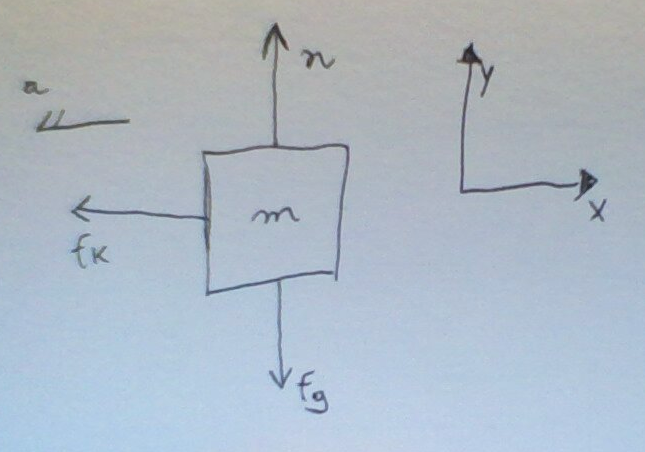
\includegraphics[scale=0.4]{hw6_problem9_fbd}
			\caption{Free-Body Diagram (Problem 9)}
			\label{fig:hw6_problem9_fbd}
		\end{center}
	\end{figure}

	\begin{align}
		f_{k} = \ &\mu_{k}n& \notag
	\end{align}

	Newton's $2^{nd}$ Law to discover $n$:

	\begin{align}
		\sum F_{y} = \ &ma_{y}& \notag \\
		n - mg = \ &m(0)& \notag \\
		n = \ &mg& \notag
	\end{align}

	\begin{align}
		\mu_{k} = \ &\frac{f_{k}}{mg}& \notag \\
		= \ &\frac{440 \ N}{(79 \ kg)\left( 9.80 \ m/s^{2} \right)}& \notag \\
		= \ &0.568&
	\end{align}
